
\chapter{Industrial Context and State of the Art}

\section{Introduction}

Autonomous yard-logistics systems integrate industrial transport, automated driving, remote supervision, and changing environmental conditions. Evaluating their performance requires considering more than the vehicle alone. It must also account for the logistics process, operational constraints, and available data. This chapter therefore examines the industrial context and relevant state of the art.

It first presents the host company and project environment. It then describes the autonomous yard-logistics system, its operating area, system actors, transfer workflow, mission phases, architecture, and data sources.

The theoretical foundations of Overall Equipment Effectiveness are then reviewed. The discussion focuses on its classical model, applications beyond manufacturing, and limitations for autonomous systems. The chapter also examines autonomous-vehicle metrics, ODD, SOTIF, reliability indicators, and process capability. Finally, the chapter identifies the research gap and presents the project methodology.

\section{Industrial and Project Context}

\subsection{Presentation of TII KAMAG}

This graduation project was carried out at TII KAMAG, a subsidiary of the TII Group (Transporter Industry International Group), a globally recognized manufacturer of heavy-duty transport vehicles and specialized logistics solutions. Founded in 1969, TII KAMAG 
has evolved from a small engineering company into a leading provider of innovative transport systems designed to meet the demanding requirements of heavy industries.\cite{tiikamag_linkedin} \cite{tiikamag_website}
\begin{figure}[H]
    \centering

    \begin{minipage}{0.45\textwidth}
        \centering
        
\includegraphics[width=0.7\linewidth]{images/tii-kamag-logo.png}
        \captionof{figure}{TII KAMAG Logo}
        \label{fig:tii-kamag-logo}
    \end{minipage}
    \hfill
    \begin{minipage}{0.45\textwidth}
        \centering
        
\includegraphics[width=0.7\linewidth]{images/tii-group.png}
        \captionof{figure}{TII Group Logo}
        \label{fig:tii-group-logo}
    \end{minipage}

\end{figure}
TII KAMAG operates in several industrial domains, including automotive, aerospace, and logistics solutions for heavy-goods transport.
As a transport-technology provider, the company is developing autonomous driving systems to improve logistics processes in heavy industry.
This work follows two complementary directions: improving existing vehicle systems and developing solutions that can perform complex tasks autonomously in demanding environments. \\
TII KAMAG offers a range of industrial transport solutions, focusing on advanced logistics and material-handling applications. One key product, the Kamag Precision Tractor, is a specialized terminal vehicle for transport and handling operations in logistics environments. The Kamag Precision Mover complements this solution by handling and transporting swap bodies and semi-trailers within logistics hubs and industrial yards. Logistics companies such as DACHSER have used this application for many years, demonstrating its industrial relevance. \cite{tiikamag_website} \\

These vehicles reflect TII KAMAG’s focus on intelligent technologies and autonomous driving to improve efficiency and reliability in demanding environments. The company also provides fleet management, operator training, and maintenance services to support reliable operation for its international customers.


\begin{figure}[H]
    \centering
  \begin{minipage}{0.4\textwidth}
        \centering
        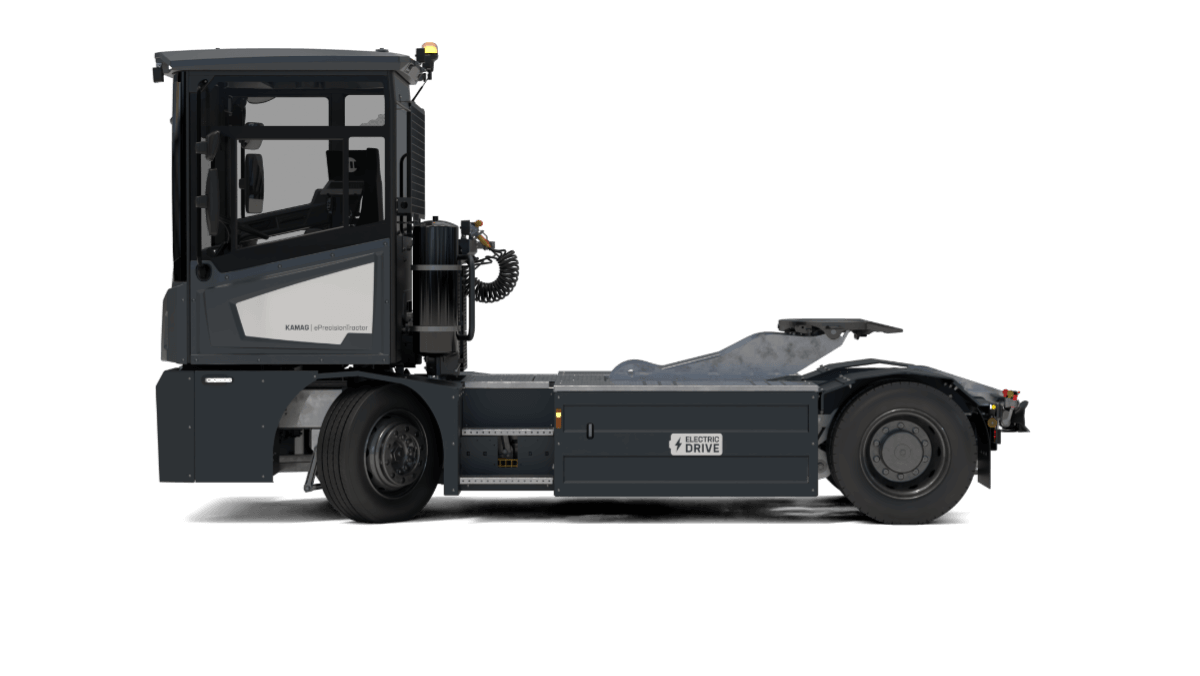
\includegraphics[width=\linewidth]{images/PrecisionTractor.png}
    \captionof{figure}{Kamag Precision Tractor\cite{tiikamag_website}}
        \label{fig:precision_tractor}
  \end{minipage}
    \hfill
  \begin{minipage}{0.4\textwidth}
        \centering
        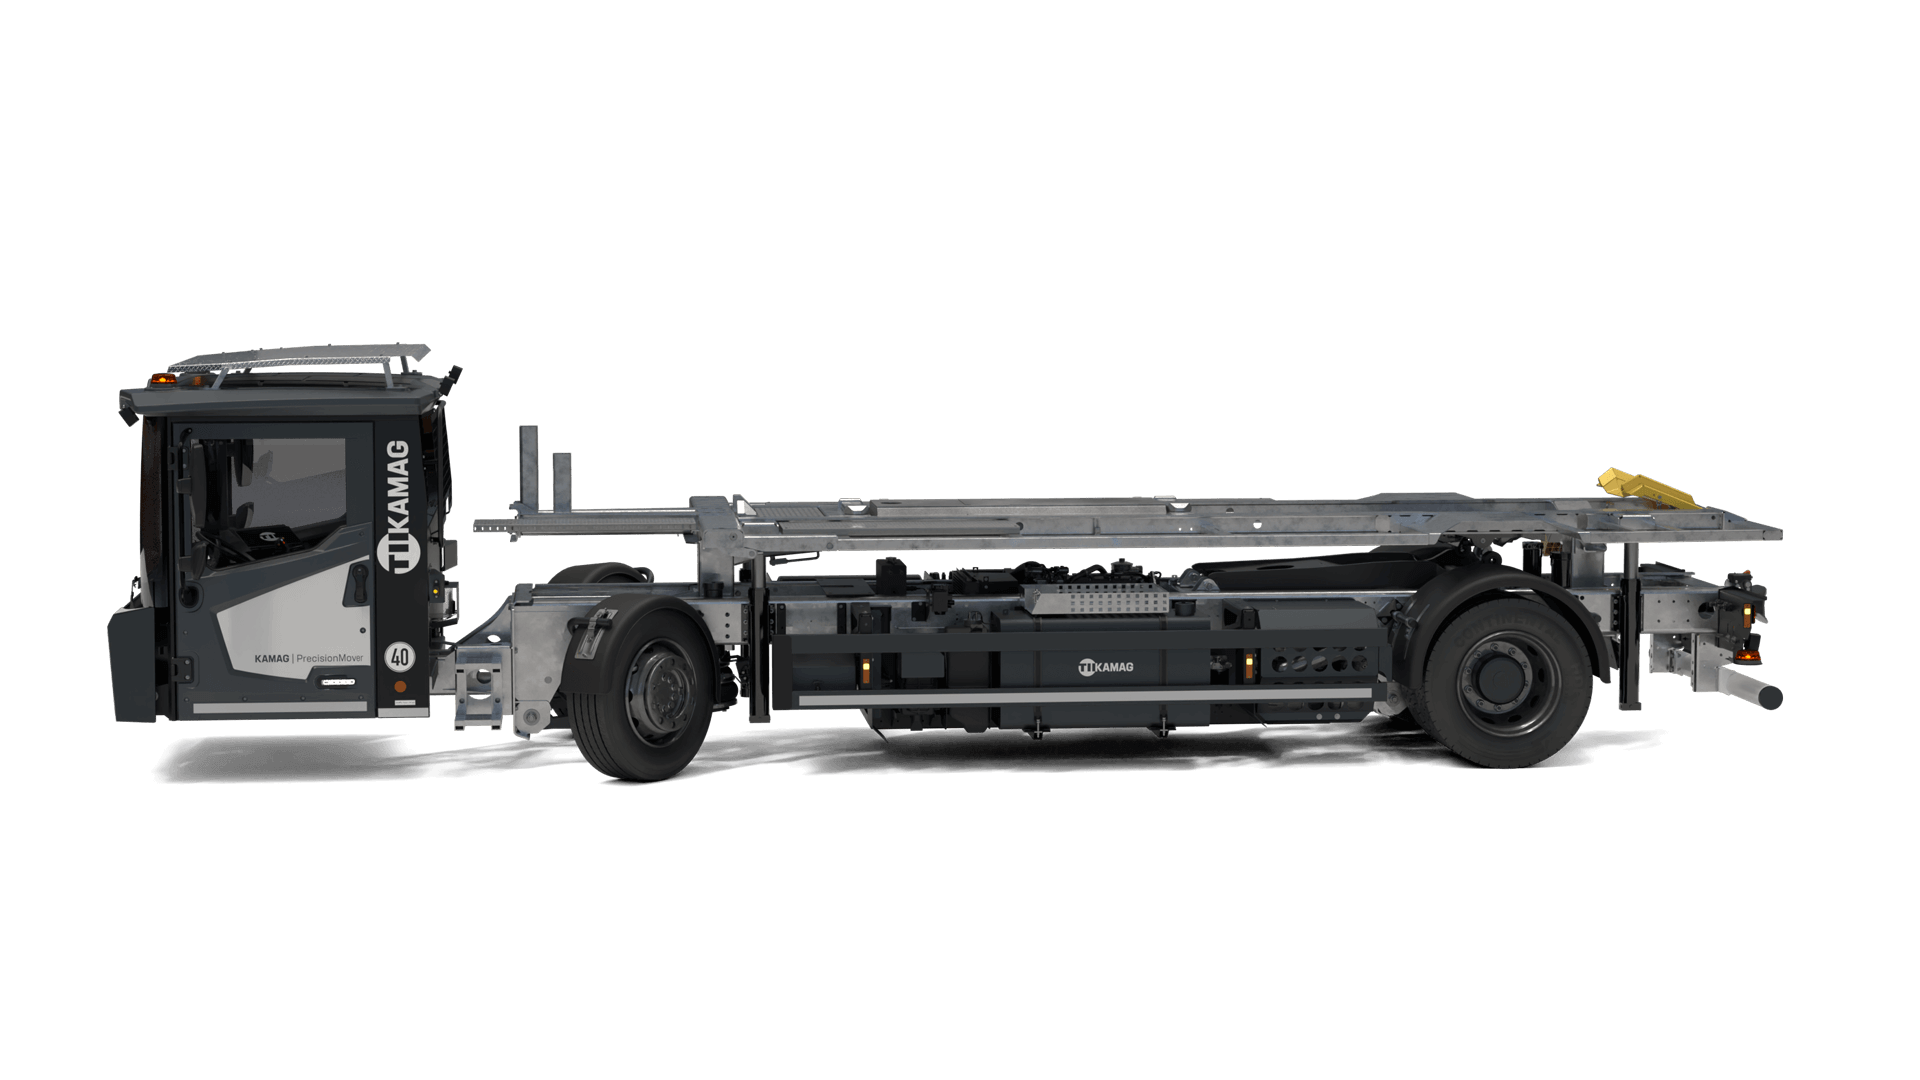
\includegraphics[width=\linewidth]{images/PrecisionMover.png}
    \captionof{figure}{Kamag Precision Mover\cite{tiikamag_website}}
        \label{fig:precision_mover}
  \end{minipage}

\end{figure}

TII KAMAG operates from an industrial site comprising multiple production facilities and technical departments dedicated to the development of transport technologies. The company employs approximately 350 people who contribute to the design, manufacturing, and continuous improvement of specialized transport solutions for customers worldwide.
\begin{figure}[H]
    \centering
  \begin{minipage}{0.48\textwidth}
        \centering
        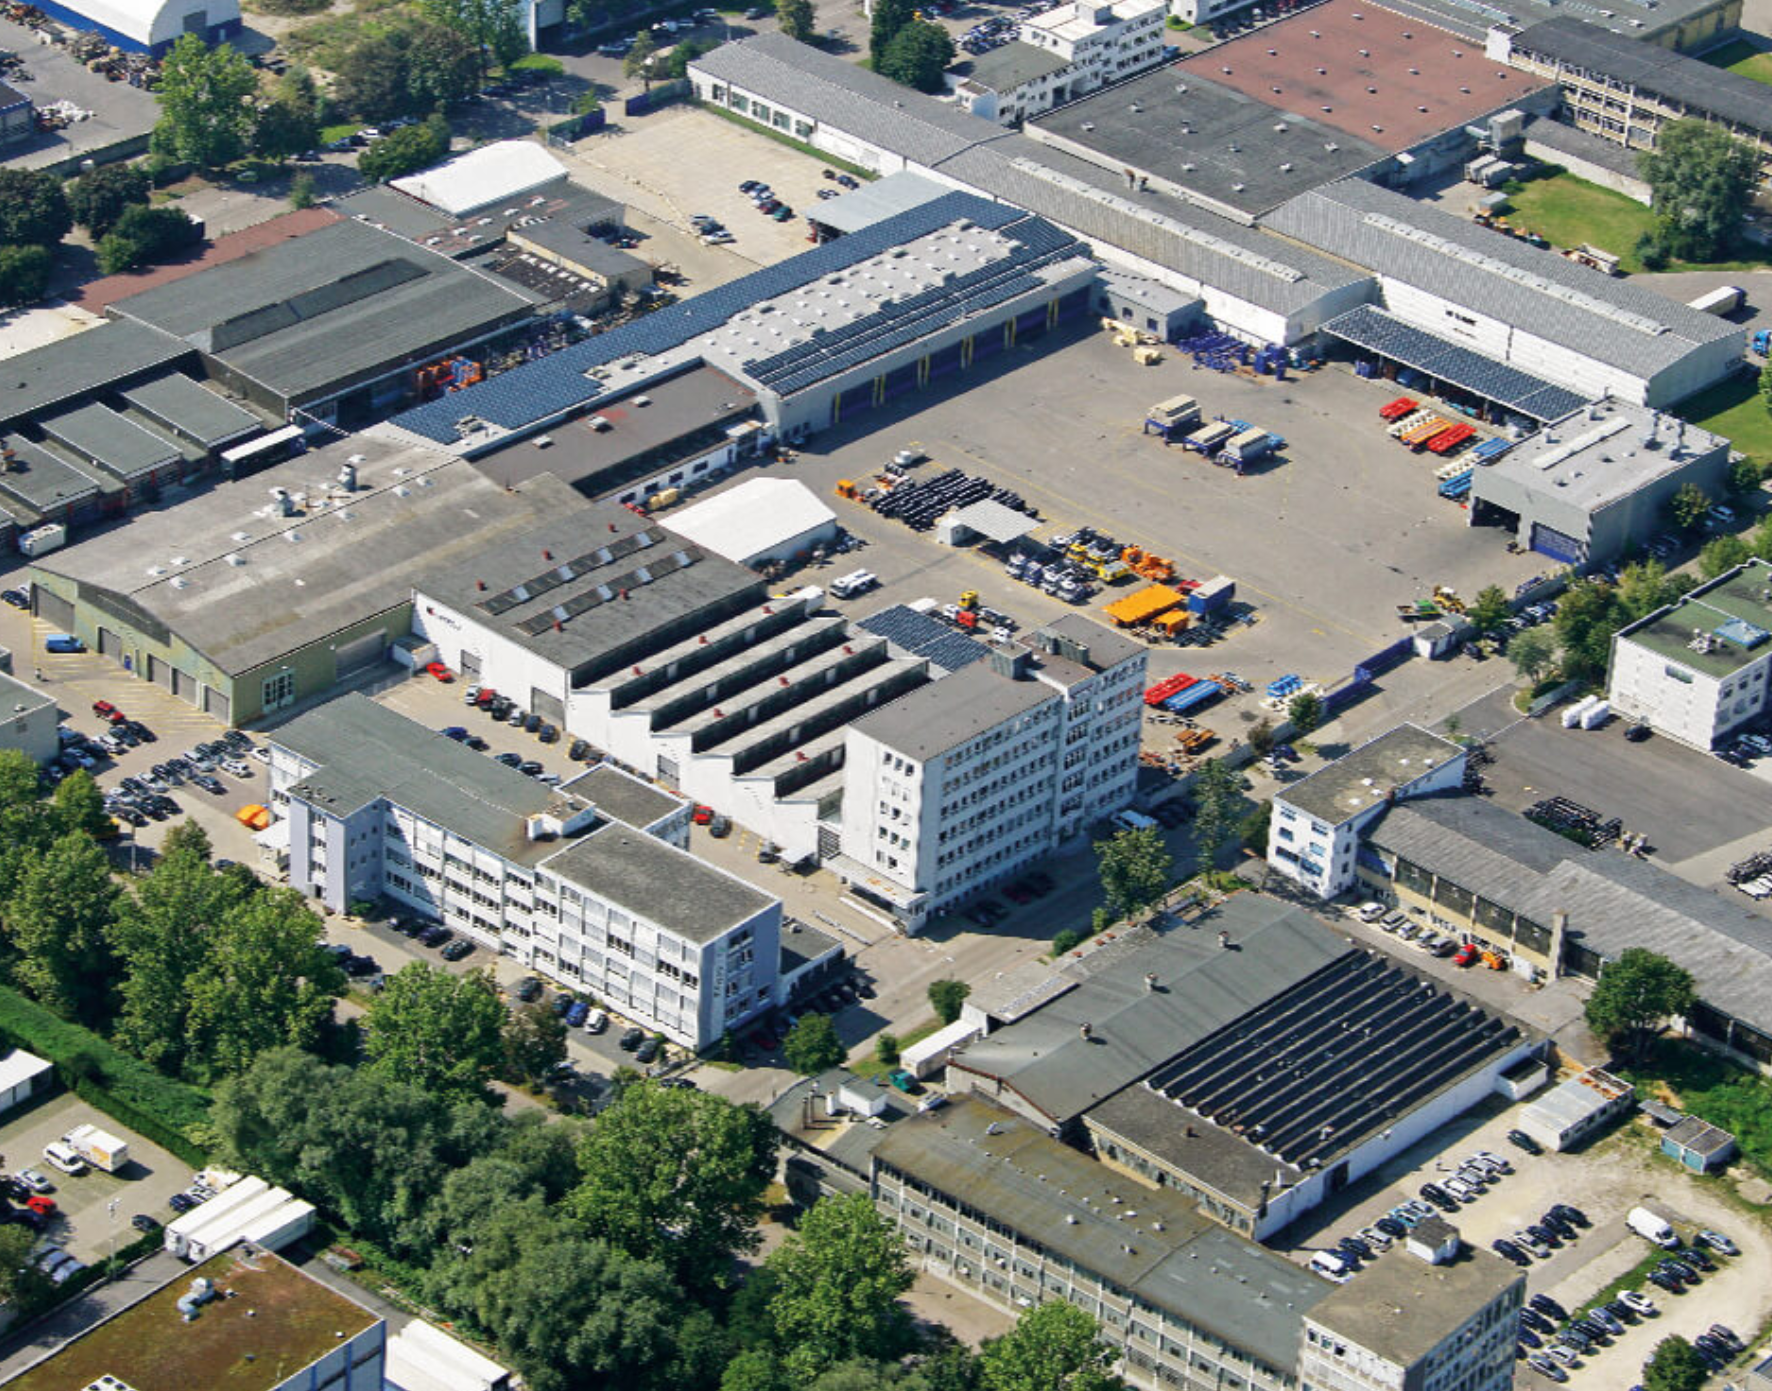
\includegraphics[width=\linewidth]{images/TIIKAMAGYARD.png}  
        \captionof{figure}{TII KAMAG Campus\cite{tiikamag_website}}
        \label{fig:tiikamag_yard}
  \end{minipage}
\end{figure}


\subsection{Project Context and Objectives}

The development of autonomous transport solutions creates a need for suitable methods to evaluate their operational effectiveness. Unlike stationary production equipment, autonomous yard vehicles execute variable transport missions under changing traffic and environmental conditions. These characteristics make the direct application of classical OEE insufficient for identifying and interpreting the main sources of operational loss.

Within this industrial context, the objective of this graduation project is to \textbf{design and implement an \gls{oee}-based performance measurement framework adapted to autonomous yard logistics}. The work aims to define suitable Availability, Performance, and Quality metrics, account for \GLS{odd}-related constraints. It also provides complementary indicators for deeper operational diagnosis. The framework is supported by a structured data model and implemented using the available operational data.

\section{Autonomous Yard-Logistics System}
\label{sec:industrial-operating-context}

The system under study operates within the DACHSER yard, where autonomous vehicles perform swap body transfer operations in a defined industrial logistics area.

\subsection{Operating Environment and System Actors}

The yard is a semi-structured environment with predefined driving paths connecting multiple parking locations. Parking locations may contain swap bodies, standardized load units supported by folding legs, or no load unit. The area is shared with pedestrians and manually operated vehicles, so the autonomous system must navigate intersections, crossing areas, and changing operational conditions.

Three actors are involved in the operation: the autonomous Kamag Precision Mover, which executes transport missions; the remote supervisor or safety operator, who monitors operation, manages protective stops, validates specific manoeuvres, and intervenes when necessary; and the yard operations team, which manages transport orders, mission coordination, and operational exceptions.

\subsection{Swap Body Transfer Workflow}

The transfer is the basic unit of operation and represents the relocation of one swap body from a source location to a destination location. It may involve two missions: a pick-up mission, during which the Kamag Precision Mover travels to the source location, positions itself beneath the swap body, and lifts it; and a set-down mission, during which the loaded vehicle transports the swap body to the destination and unloads it.

\begin{figure}[H]
  \centering
  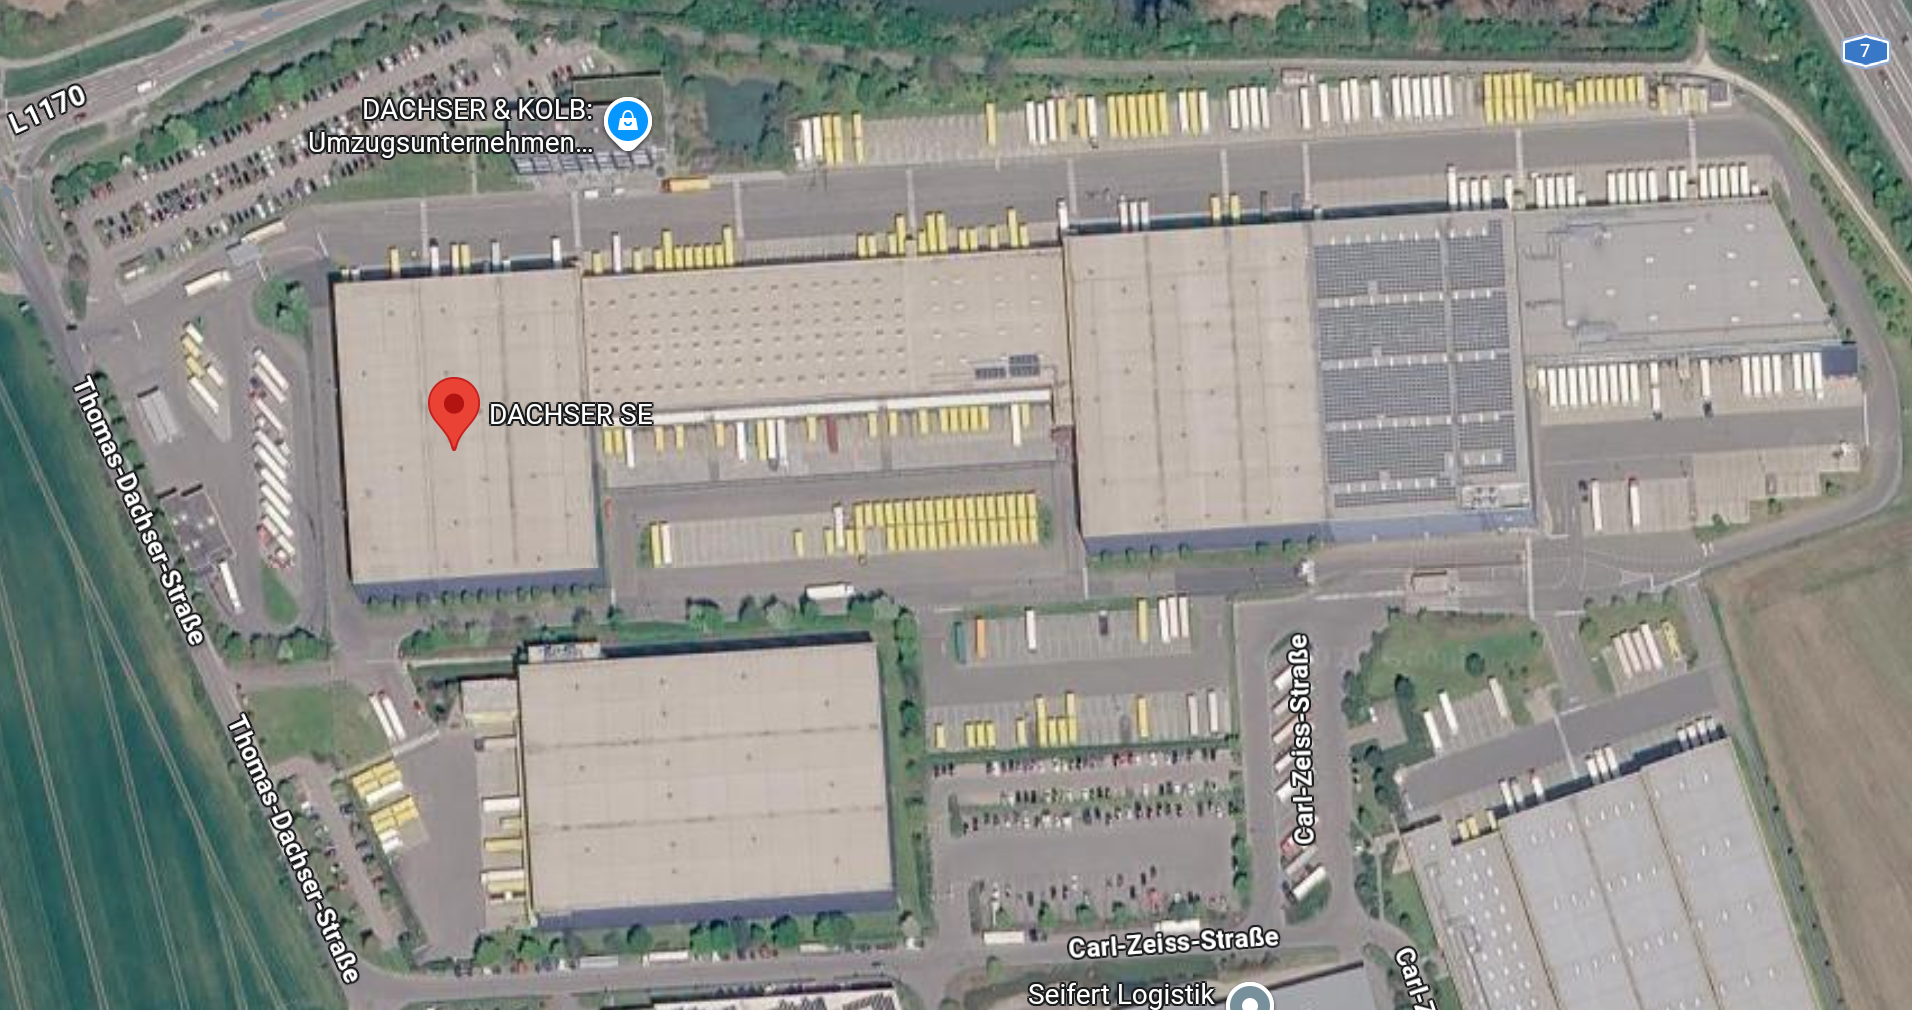
\includegraphics[width=0.7\textwidth]{images/dachseryard.png}
  \caption[The Dachser Yard]{The Dachser Yard~\cite{dachser_google_maps}}
  \label{fig:dachseryard}
\end{figure}
\subsection{Operational Hierarchy}
The logistics operation is structured into three levels: transfer, mission, and mission phase. A transfer represents the complete transport order from a source location to a destination. It is composed of one or two missions depending on the transfer scenario. Each mission describes a specific part of the transport operation, such as pick-up, set-down, or repositioning. Missions are further decomposed into elementary mission phases that describe the individual actions executed by the vehicle.
\subsection{Mission Phases and Transfer Scenarios}

The vehicle operation is divided into eight mission phases, denoted MP1 to MP8. These phases cover path following, manoeuvring, insertion, load handling, extraction, and return to the predefined path. Table \ref{tab:mission-phases} summarises their definitions, while Figure \ref{fig:MPdesc} illustrates the phase sequence.

\begin{figure}[H]
  \centering
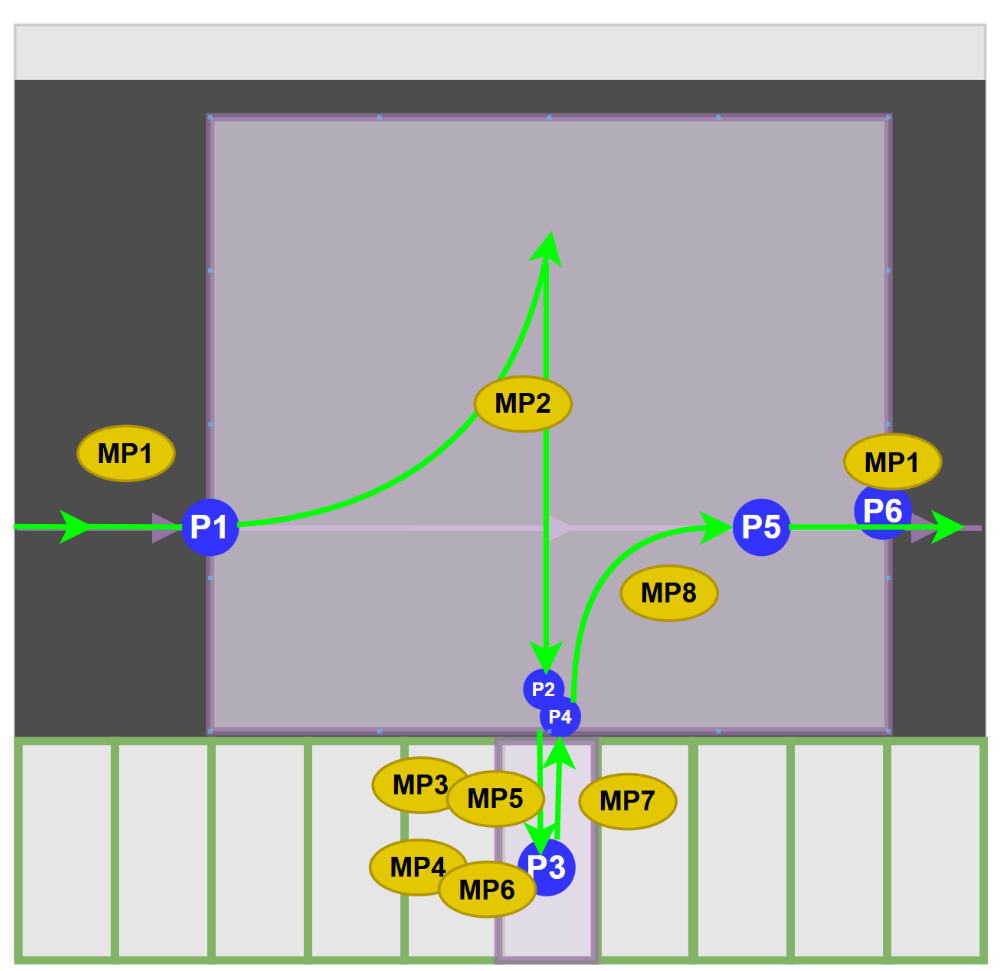
\includegraphics[width=0.7\textwidth]{images/MPdesc.png}
\caption{Mission Phases Representation}
\label{fig:MPdesc}
\end{figure}

\begin{table}[H]
  \centering
  \caption{Canonical Mission Phases}
  \label{tab:mission-phases}
  \begin{adjustbox}{max width=\textwidth}
    \begin{tabular}{|c|p{4.3cm}|c|p{5.8cm}|}
      \hline
      \textbf{Phase} & \textbf{Description} & \textbf{Navigation mode} & \textbf{Detailed description} \\
      \hline
      MP1 & Follow the predefined path & follower & The \gls{av} drives forward or backward along the predefined path to \textbf{P1} \\
      \hline
      MP2 & Manoeuvre toward pre-insertion point & manoeuvre & From \textbf{P1} to \textbf{P2} \\
      \hline
      MP3 & Insert into spot under swap body & manoeuvre & From \textbf{P2} to \textbf{P3} \\
      \hline
      MP4 & Pick up swap body & manoeuvre & At \textbf{P3} \\
      \hline
      MP5 & Insert into empty spot & manoeuvre & From \textbf{P2} to \textbf{P3} \\
      \hline
      MP6 & Set down swap body & manoeuvre & At \textbf{P3} \\
      \hline
      MP7 & Extract from spot & manoeuvre & From \textbf{P3} to \textbf{P4} \\
      \hline
      MP8 & Catch up the predefined path & manoeuvre & From \textbf{P4} to \textbf{P5} \\
      \hline
    \end{tabular}
  \end{adjustbox}
\end{table}

A transfer is classified by whether each of its two missions requires long-distance travel or takes place in close proximity to the target spot:

\begin{table}[H]
  \centering
  \caption{Transfer scenarios}
  \label{tab:transfer-scenarios}
  \renewcommand{\arraystretch}{1.2}
  \begin{tabular}{|p{3cm}|p{11cm}|}
      \hline
      \textbf{Scenario} & \textbf{Mission-phase sequence} \\
      \hline
      \textbf{classic} &
      \parbox[t]{\linewidth}{\textbf{Mission 1: PICK\_UP}\\ MP7 $\rightarrow$ MP8 $\rightarrow$ MP1 $\rightarrow$ MP2 $\rightarrow$ MP3 $\rightarrow$ MP4\\[0.2em]
      \textbf{Mission 2: SET\_DOWN}\\ MP7 $\rightarrow$ MP8 $\rightarrow$ MP1 $\rightarrow$ MP2 $\rightarrow$ MP5 $\rightarrow$ MP6} \\
      \hline
      \textbf{Close proximity pick up} &
      \parbox[t]{\linewidth}{\textbf{Mission 1: CLOSE\_PROXIMITY\_PICK\_UP}\\ MP7 $\rightarrow$ MP2 $\rightarrow$ MP3 $\rightarrow$ MP4\\[0.2em]
      \textbf{Mission 2: SET\_DOWN}\\ MP7 $\rightarrow$ MP8 $\rightarrow$ MP1 $\rightarrow$ MP2 $\rightarrow$ MP5 $\rightarrow$ MP6} \\
      \hline
      \textbf{Close proximity set down} &
      \parbox[t]{\linewidth}{\textbf{Mission 1: PICK\_UP}\\ MP7 $\rightarrow$ MP8 $\rightarrow$ MP1 $\rightarrow$ MP2 $\rightarrow$ MP3 $\rightarrow$ MP4\\[0.2em]
      \textbf{Mission 2: CLOSE\_PROXIMITY\_SET\_DOWN}\\ MP7 $\rightarrow$ MP2 $\rightarrow$ MP5 $\rightarrow$ MP6} \\
      \hline
      \textbf{Double close proximity} &
      \parbox[t]{\linewidth}{\textbf{Mission 1: CLOSE\_PROXIMITY\_PICK\_UP}\\ MP7 $\rightarrow$ MP2 $\rightarrow$ MP3 $\rightarrow$ MP4\\[0.2em]
      \textbf{Mission 2: CLOSE\_PROXIMITY\_SET\_DOWN}\\ MP7 $\rightarrow$ MP2 $\rightarrow$ MP5 $\rightarrow$ MP6} \\
      \hline
      \textbf{park (GO\_TO)} &
      \parbox[t]{\linewidth}{\textbf{Mission 1: GO\_TO}\\ MP7 $\rightarrow$ MP8 $\rightarrow$ MP1 $\rightarrow$ MP2 $\rightarrow$ MP5\\[0.2em]
      \textit{Single mission scenario}} \\
      \hline
    \end{tabular}
  \renewcommand{\arraystretch}{0.85}
\end{table}

\subsection{System and Data Architecture}

The autonomous yard logistics system consists of two layers: an onboard vehicle layer and an off-board data-management layer. During transport missions, the \gls{av} continuously generates data on vehicle states, mission execution, events, and outcomes.

At the vehicle level, onboard logging records each mission's operational trace, including timestamps, mission phases, system events, and execution results. These records support the reconstruction of transport operations and the identification of performance losses.

The telemetry data is transmitted to off-board systems, where fleet information is consolidated into an Automatic Telemetry Dataset. This dataset provides the main input for computing \glspl{kpi} and evaluating \gls{oee}.

This architecture links autonomous operation to performance analysis: vehicle execution generates operational data, telemetry systems collect and organize it, and the resulting dataset supports the evaluation of autonomous yard effectiveness.
\begin{figure}[H]
  \centering
  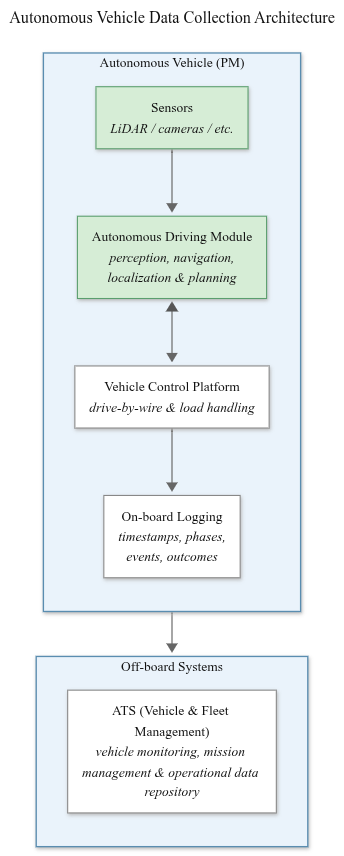
\includegraphics[width=0.3\textwidth]{images/System Architecture.png}
  \caption{System Architecture}
  \label{fig:systemarchitecture}
\end{figure}

\subsection{Available Data and Evaluation Constraints}

This section describes the data foundation used to design and evaluate the proposed performance measurement framework.
\begin{itemize}
  \item \textbf{Data sources:} The framework relies on two complementary data sources. The first is the automatic dataset, generated from vehicle operation and containing machine-recorded information such as timestamps, mission phases, operational events, and execution outcomes. The second is a manual field log maintained by operators, providing additional contextual information regarding interventions, exceptions, and operational events that cannot always be fully captured through automatic telemetry alone. These two sources are combined at the transfer level to create a unified structured dataset representing each transport operation. Real operational data from both sources was analysed during the design phase to identify the data fields and input structure required by the proposed framework, and to validate that the necessary information is practically collectable from the system.


  \item \textbf{Historical and synthetic data:} Due to limitations in data coverage and completeness, real records alone were insufficient for a comprehensive evaluation. A synthetic dataset was therefore generated following the same input schema derived from the real data, enabling controlled and reproducible testing of the framework under predefined performance scenarios while remaining consistent with real operational characteristics.
\end{itemize}
\begin{figure}[H]
  \centering
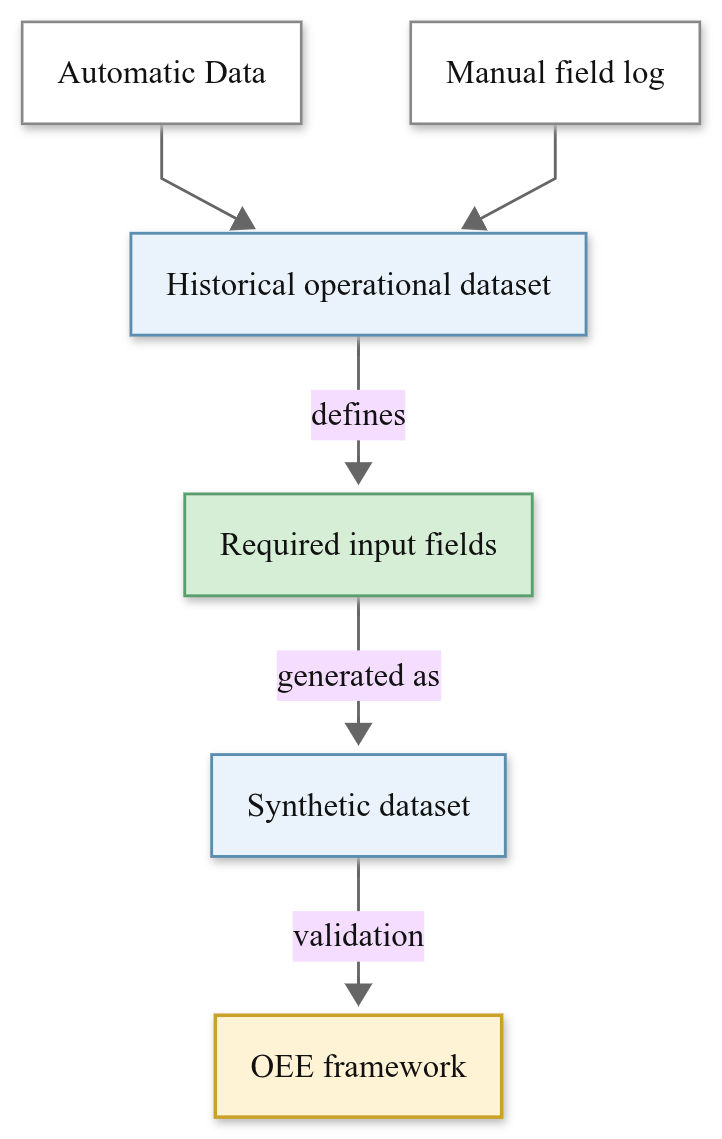
\includegraphics[width=0.4\textwidth]{images/Data provenance flow.png}
\caption{Data Provenance Flow}
\label{fig:datacollectioncontext}
\end{figure}


\section{Industrial Performance-Measurement Problem}

\gls{oee} was developed to evaluate stationary manufacturing equipment operating under repetitive and predictable conditions. Its classical formulation assumes fixed production cycles, clearly defined operating states, and losses categorized as availability, performance, and quality. Under these conditions, \gls{oee} effectively measures equipment utilization and production efficiency.

These assumptions do not fully apply to \glspl{av} operating in dynamic yard environments. Unlike industrial machines, \gls{av} missions are affected by travel distances, route configurations, traffic, loading and unloading operations, and interactions with people and infrastructure. Operational interruptions also cannot always be interpreted as equipment failures. An \gls{av} may stop because of safety constraints, remote-supervision requests, autonomy limitations, congestion, or environmental conditions while remaining technically functional.

Applying conventional \gls{oee} to autonomous yard operations may therefore obscure the true causes of performance losses by grouping fundamentally different events into identical categories. Mechanical failures, autonomy-related limitations, safety interventions, and environmental constraints require separate interpretation to support effective operational decisions.

Current autonomous-driving metrics, such as disengagement rate and intervention frequency, primarily evaluate autonomy and safety. However, they do not measure the overall effectiveness of logistics operations. Traditional \gls{oee}, measures equipment efficiency but lacks the operational states and loss categories required for autonomous vehicles. This creates a measurement gap: existing approaches cannot precisely determine the useful transport work performed by an autonomous fleet.

A dedicated performance-measurement framework is therefore required for autonomous yard logistics. Such a framework should preserve the industrial relevance of \gls{oee} while adapting its time hierarchy, performance indicators, and loss classification to mission variability, autonomy-specific events, supervision requirements, and operational constraints. This work addresses this need by developing an \gls{oee}-based performance-measurement approach for the autonomous transport system deployed in the DACHSER yard.

\section{Overall Equipment Effectiveness Foundations}

This section presents the foundations of \gls{oee} and its relevance to autonomous yard logistics. It reviews the classical \gls{oee} framework, its extension beyond manufacturing, and the assumptions underlying its main factors. It also introduces the Six Big Losses and relevant industrial standards. These foundations provide the basis for identifying the limitations that motivate the adapted framework proposed in this work.
\subsection{Origins and Rationale of OEE}
 \gls{oee} is a key manufacturing metric used to quantify production efficiency by identifying and reducing operational losses. Seiichi Nakajima introduced the concept in 1988 as part of Total Productive Maintenance (\gls{tpm}), a methodology developed by the Japan Institute of Plant Maintenance.\cite{nakajima1988tpm} The objective of \gls{tpm} is to maximize equipment effectiveness throughout its lifecycle through a comprehensive maintenance system involving all departments and employees.

Nakajima's work provided a structured method for evaluating equipment performance beyond simple uptime. OEE combines equipment availability, operating speed, and product quality to reveal the capacity lost through inefficiencies. This lost capacity is often described as the ``Hidden Factory.'' By separating overall effectiveness into distinct factors, OEE supports targeted improvement actions and waste reduction.
\subsection{Availability, Performance, and Quality}
OEE is calculated as the product of three factors:
\[
\mathrm{OEE} = A \cdot P \cdot Q
\]
Availability, Performance, and Quality represent different types of operational loss:
\begin{itemize}
    \item \textbf{Availability} measures the proportion of scheduled operating time during which the equipment is running. It accounts for downtime losses such as breakdowns, setups, and adjustments.
    \item \textbf{Performance} compares the actual operating speed with the ideal cycle time. It accounts for losses caused by minor stops and reduced speed.
    \item \textbf{Quality} measures the proportion of good products in the total output. It accounts for losses caused by defects and rework.
\end{itemize}
\subsection{Fixed-Cycle Assumption}
Classical OEE relies on a fixed-cycle assumption. For a given product, the ideal production cycle is assumed to remain constant. This cycle provides the reference for measuring actual operating speed and calculating the Performance factor. Deviations from the ideal cycle, including minor stops and reduced speed, are therefore classified as performance losses.

This assumption is effective in stable and repetitive manufacturing environments. However, it becomes difficult to apply to dynamic systems whose mission durations and operating conditions vary. This limitation is particularly important when extending OEE to autonomous vehicles.
\subsection{The Six Big Losses}
Nakajima's OEE framework classifies production inefficiencies into the ``Six Big Losses.''\cite{nakajima1988tpm} This taxonomy provides a structured method for identifying the main causes of equipment underutilization:
\begin{enumerate}
    \item \textbf{Equipment Failure (Availability Loss):} unplanned downtime caused by breakdowns or technical faults.
    \item \textbf{Setup and Adjustment (Availability Loss):} planned downtime required to prepare the machine for a different production run.
    \item \textbf{Idling and Minor Stops (Performance Loss):} brief interruptions or jams that temporarily stop production.
    \item \textbf{Reduced Speed (Performance Loss):} operation at a speed below the theoretical maximum.
    \item \textbf{Process Defects (Quality Loss):} scrap or defective parts produced during steady-state operation.
    \item \textbf{Reduced Yield (Quality Loss):} defective parts produced during startup or production transitions.
\end{enumerate}
The Six Big Losses are highly effective for static and repetitive manufacturing processes because they provide a clear structure for continuous improvement. However, their direct application to autonomous yard logistics requires adaptation to mobile operation, variable missions, and autonomy-related events.
\begin{figure}[H]
   \centering
  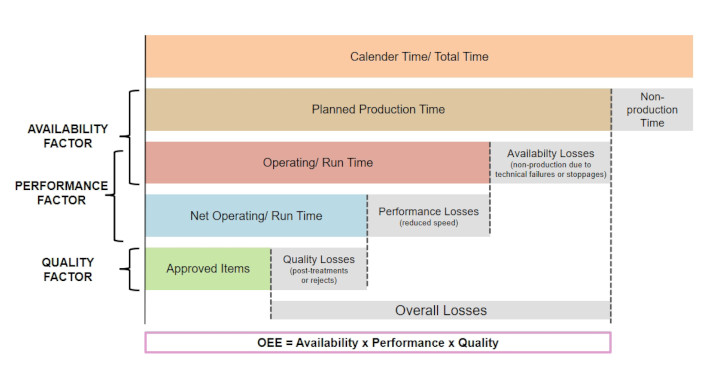
\includegraphics[width=0.8\textwidth]{images/Time-model-for-OEE-measuring.jpg}
  \caption[Major Losses and Computation of OEE]{Major Losses and Computation of OEE\cite{sciencedirect_oee_figure}}
  \label{fig:hard}
\end{figure}
\subsection{Industrial Standards and Guidelines}
Several standards and industrial guidelines support the consistent definition and measurement of OEE-related indicators:
\begin{itemize}
  \item \textbf{ISO 22400-2:2014:} This standard defines KPIs for manufacturing operations management. It provides formal definitions for indicators such as Availability, which is calculated as the ratio of Operating Time to Planned Production Time.\cite{iso22400_2_2014}

  \item \textbf{SEMI E10:} Developed for the semiconductor industry, this standard defines equipment states and provides a framework for measuring reliability, availability, and maintainability (\gls{ram}). It distinguishes states such as Productive, Standby, and Unscheduled Downtime.\cite{semi_e10_ram} SEMI E79 extends this framework to define OEE for semiconductor manufacturing equipment.

  \item \textbf{VDMA guidelines:} Guidelines such as VDMA 66412 support the standardization of manufacturing execution system (\gls{mes}) KPIs. They are generally aligned with ISO 22400 and provide guidance for data collection and analysis, with particular emphasis on technical availability.
\end{itemize}
\section{OEE Beyond Manufacturing}
While OEE originated in discrete manufacturing, its underlying principles of identifying, classifying, and quantifying operational losses have gradually been extended to other industrial domains. As automation has expanded beyond traditional production lines, researchers have explored the application of OEE to logistics, warehousing, and mobile robotic systems. Although the fundamental objective remains the maximization of asset effectiveness, the transition from stationary production equipment to mobile autonomous systems requires substantial adaptation of both performance indicators and loss definitions.
\subsection{OEE in Logistics and Material-Handling Systems}
The application of OEE has progressively expanded from manufacturing equipment to automated material handling systems, including conveyor systems, sorting equipment, \glspl{agv}, and \glspl{amr}. These technologies play an increasingly important role in modern intralogistics by automating material transportation and improving operational efficiency.

\subsection{Adaptation of OEE Components to Mobile Systems}
Existing research shows that the three classical OEE dimensions remain applicable to mobile robotic systems, but require reinterpretation. Availability reflects vehicle readiness and downtime, Performance focuses on mission execution efficiency and speed, and Quality considers successful and error-free mission completion. Thus, OEE shifts from measuring machine productivity to evaluating the effectiveness and utilization of autonomous material handling systems~\cite{fragapane2021intralogistics}.
\begin{figure}[H]
   \centering
  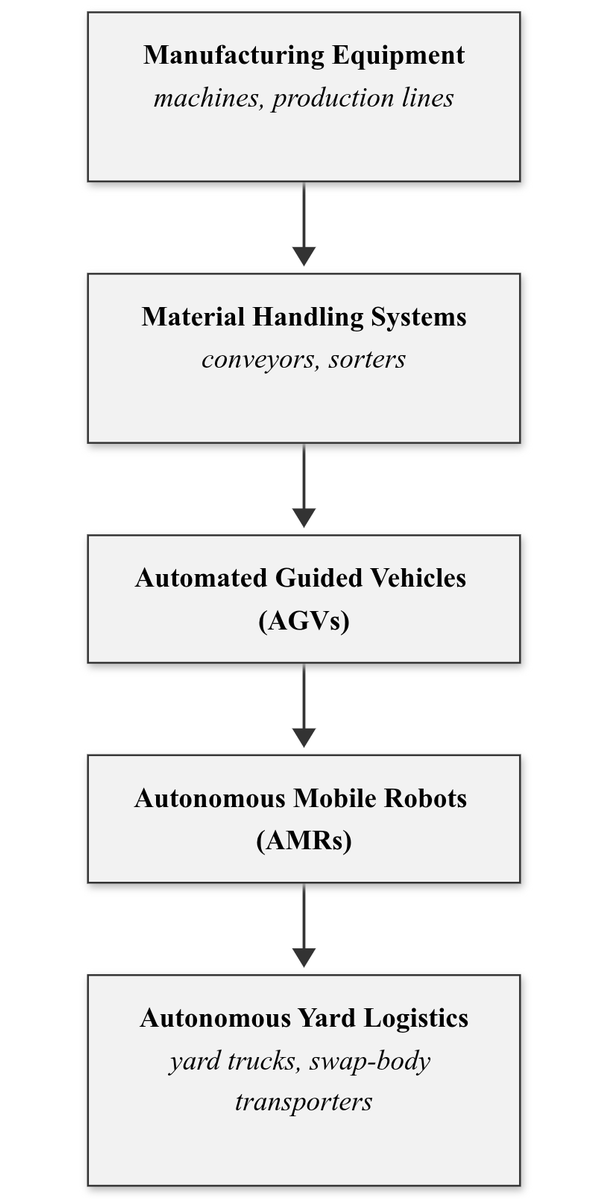
\includegraphics[width=0.3\textwidth]{images/oee_evolution.png}
  \caption[Evolution of OEE applications]{Evolution of OEE applications in logistics and mobile robotic systems.}
  \label{fig:oee-evolution}
  
\end{figure}
\subsection{Adaptation of the Six Big Losses}
Applying \gls{oee} to mobile logistics also requires reinterpreting Nakajima's Six Big Losses. The original loss taxonomy was developed for stationary production equipment. Therefore it does not adequately represent the operational characteristics of autonomous mobile systems operating in dynamic environments.

Within \glspl{agv} and \glspl{amr} applications, traditional setup and adjustment losses are commonly associated with battery refueling, software updates, vehicle initialization, or task assignment procedures. Idling and minor stoppages are frequently caused by obstacle avoidance, traffic congestion, waiting at intersections, or temporary interactions with human operators. Reduced speed losses arise when vehicles intentionally decrease their speed due to safety constraints, congestion, or navigation requirements. Likewise, process defects are reinterpreted as failed missions, misplaced loads, delivery inaccuracies, or navigation errors requiring manual intervention or mission repetition.

These adaptations demonstrate that although the philosophy of loss identification remains applicable, the nature of the losses changes significantly when moving from fixed manufacturing equipment to autonomous mobile systems. Consequently, several studies emphasize the need for specialized loss taxonomies that accurately represent the operational behavior of autonomous logistics vehicles.
\begin{table}[!ht]
\renewcommand{\arraystretch}{1.5}
\centering
\caption{Adaptation of Nakajima's Six Big Losses to Mobile Logistics}
\label{tab:mobile-logistics-losses}
\begin{tabular}{|p{5cm}|p{9cm}|}
\hline
\textbf{Classical Six Big Loss} & \textbf{Mobile Logistics Interpretation} \\
\hline
Equipment failures & Vehicle hardware or software failures \\
\hline
Setup and adjustment & Battery refueling, software updates, vehicle initialization, task assignment \\
\hline
Idling and minor stops & Obstacle avoidance, traffic congestion, waiting at intersections or doors \\
\hline
Reduced speed & Speed reduction due to safety constraints, congestion, or navigation \\
\hline
Process defects & Failed missions, misplaced loads, delivery errors, navigation failures \\
\hline
Startup losses & Localization, calibration, or system initialization errors \\
\hline
\end{tabular}
\end{table}
\subsection{Limitations of OEE for Autonomous Systems}

Despite these adaptations, applying classical \gls{oee} directly to autonomous systems remains challenging, particularly in outdoor logistics environments. Autonomous vehicles differ from conventional manufacturing equipment in several ways, which complicates the interpretation of the traditional \gls{oee} factors.

First, autonomous vehicles operate in changing environments affected by traffic, weather, pedestrians, and interactions with other vehicles. Unlike production machines operating under controlled conditions, variations in mission duration may result from environmental conditions rather than equipment inefficiency.

Second, the fixed-cycle assumption of classical \gls{oee} is difficult to apply. Mission durations vary with travel distance, route complexity, traffic, obstacle avoidance, and operational priorities. As a result, defining a single ideal cycle time as a meaningful performance benchmark is difficult.

Finally, autonomous systems generate operational events that have no direct equivalent in conventional manufacturing. Human interventions, remote-operator takeovers, disengagements, and autonomous decision-making failures represent additional loss categories that the traditional \gls{oee} framework does not adequately capture. These events affect operational effectiveness and must therefore be considered when adapting \gls{oee} to autonomous vehicles.
\section{Performance Measurement of Autonomous Vehicles}
Evaluating autonomous vehicles requires a broader perspective than traditional indicators such as speed, fuel consumption, and travel distance. In industrial environments, performance depends on the vehicle's ability to execute assigned missions safely, reliably, and efficiently.

Unlike conventional vehicles, autonomous systems depend on the interaction between perception, decision-making, navigation, and environmental conditions. Evaluation therefore requires several frameworks and \glspl{kpi} covering autonomy, safety, reliability, and operational effectiveness.
\subsection{Levels of Driving Automation}
The SAE J3016 standard defines six levels of driving automation, ranging from Level 0 (no automation) to Level 5 (full automation). These levels describe how driving tasks are distributed between the human driver and the automated driving system.

Level 4 automation is particularly relevant to autonomous yard logistics. At this level, the \gls{ads} performs all driving tasks without human intervention within a defined \gls{odd}. Level 4 systems are therefore suitable for controlled industrial environments such as logistics yards, where operating conditions can be constrained and monitored.
\begin{figure}[H]
   \centering
  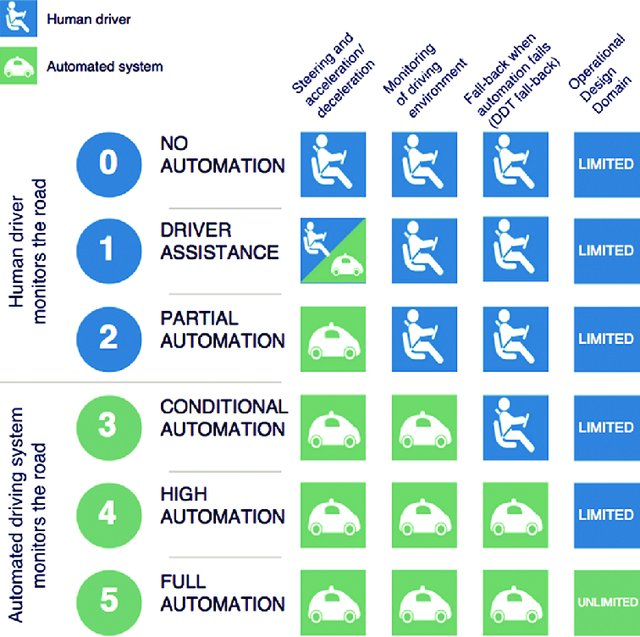
\includegraphics[width=0.4\textwidth]{images/SAE-J3016-levels-of-driving-automation_W640.jpg}
  \caption[SAE Automation Levels]{SAE Automation Levels~\cite{sae_j3016_rg}}
  \label{fig:sae-levels}
  
\end{figure}
\subsection{Autonomous-Vehicle Performance Metrics}
Autonomous vehicles are commonly evaluated using multiple \glspl{kpi}, each addressing a specific aspect of system behaviour. Unlike manufacturing systems, which often use \gls{oee} as an integrated measure of effectiveness, autonomous-vehicle research generally uses separate metrics for autonomy, safety, reliability, and operational efficiency.

Existing review studies indicate that no universally accepted framework comprehensively evaluates autonomous-vehicle performance. Most available metrics focus on individual dimensions rather than overall operational effectiveness. The main metrics used in this context are summarized in Table~\ref{tab:av-performance-metrics}.
\begin{table}[H]
\renewcommand{\arraystretch}{1.5}
\centering
\caption{Common Performance Metrics for Autonomous Vehicles}
\label{tab:av-performance-metrics}
\begin{tabular}{|p{3cm}|p{6cm}|p{5cm}|}
\hline
\textbf{KPI} & \textbf{Description} & \textbf{Performance Aspect} \\
\hline
Mission Success Rate & Percentage of missions completed successfully without failure & Mission effectiveness \\
\hline
Intervention / Disengagement Rate & Frequency of human intervention or autonomous disengagement & Autonomy and reliability \\
\hline
Technical Availability & Percentage of time the vehicle is operationally ready & System readiness \\
\hline
Mission Cycle Time & Time required to complete a transport mission & Operational efficiency \\
\hline
Fleet Utilization & Percentage of vehicles actively performing missions & Asset utilization \\
\hline
\end{tabular}
\end{table}
\subsection{Operational Design Domain}
The \gls{odd} defines the conditions under which an \gls{ads} is designed to operate safely and effectively. It describes the limits of the system's operational capability. These limits depend on environmental and operational factors. They also determine when autonomous operation can continue without human intervention.

For autonomous yard vehicles, the \gls{odd} specifies the areas in which the vehicle can operate. It also defines the conditions required for autonomous operation. These conditions include the infrastructure, road layout, weather, lighting, traffic, and presence of dynamic obstacles. They may also include speed restrictions, visibility requirements, and interaction with pedestrians or manually operated vehicles.
\subsection{ODD, SOTIF, and Performance Measurement}
ISO 34503 provides a structured approach for describing the \gls{odd} of automated driving systems. It organizes ODD characteristics into categories such as scenery, environmental conditions, and dynamic elements~\cite{iso34503_2023}.

Figure~\ref{fig:odd-components} illustrates these ODD components. Together, they define the context in which an automated driving system must operate safely. A change in any of these components may affect the vehicle's ability to continue autonomous operation.

\begin{figure}[H]
   \centering
  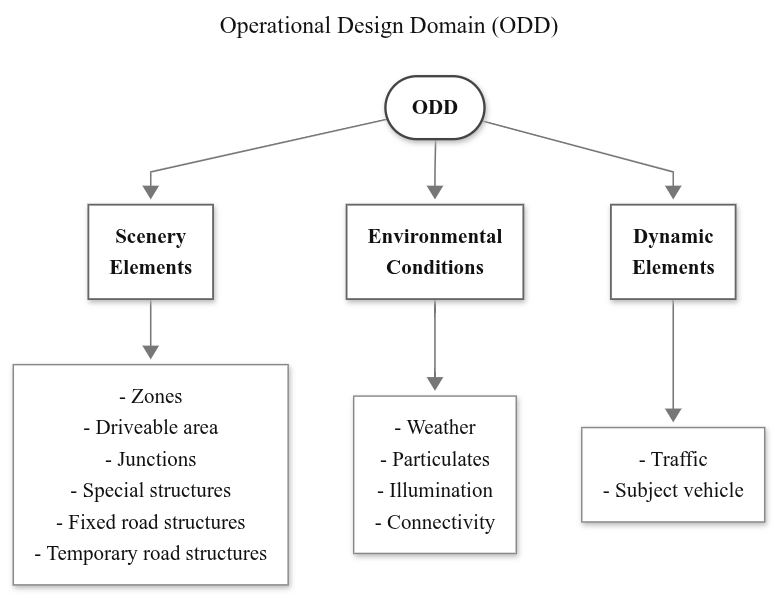
\includegraphics[width=0.6\textwidth]{images/odd_components.png}
  \caption[ODD Components]{Operational Design Domain Components~\cite{iso34503_2023}}
  \label{fig:odd-components}
\end{figure}

The \gls{sotif} concept, defined by ISO 21448, addresses safety risks caused by functional limitations of an automated system rather than hardware failures~\cite{iso21448_2022}. This concept is important for autonomous vehicles operating in complex environments, where unexpected situations may occur even when the hardware remains functional.

For example, fog or other conditions that reduce visibility may prevent an autonomous vehicle from continuing safely despite the correct operation of its hardware components.


The distinction between \gls{odd} exclusions and technical failures is therefore important. A technical failure occurs when a system component does not operate as intended, such as in the case of a sensor malfunction, communication failure, or software error. An \gls{odd} exclusion occurs when the vehicle encounters conditions outside its defined operational boundaries, such as heavy rain, dense fog, or insufficient visibility. In this case, the vehicle may remain technically functional but unable to continue autonomous operation.

This distinction affects the adaptation of \gls{oee} to autonomous vehicles. In conventional manufacturing, Availability losses are mainly associated with equipment breakdowns, maintenance, and setup activities. Autonomous vehicles introduce additional sources of unavailability related to environmental and operational constraints. ODD exclusions should therefore be treated as a distinct category of operational loss when evaluating the Availability factor.
\section{Complementary Performance Indicators}
Although OEE provides a holistic measure of operational effectiveness through the integration of Availability, Performance, and Quality, it does not fully characterize all aspects of autonomous system behaviour. In particular, reliability engineering metrics provide insight into failure behaviour and maintainability, while statistical quality methods allow the evaluation of operational consistency and variability.
\subsection{Reliability and Maintainability Metrics}
\label{sec:reliability_state_art}
Reliability engineering provides established methods for evaluating the robustness and maintainability of complex systems. For autonomous vehicles, these metrics are particularly relevant because operational effectiveness depends not only on task execution but also on the ability of the system to remain available and recover from failures.

The main reliability indicators include:

\begin{itemize}
  \item \textbf{Failure Rate ($\lambda$):} represents the frequency at which failures occur during operation. For systems with an approximately constant failure rate, it is commonly related to \gls{mtbf} as:
\end{itemize}

\[
\lambda = \frac{1}{\mathrm{MTBF}}
\]

\begin{itemize}
  \item \textbf{\gls{mtbf}:} represents the average operating time between two consecutive failures. A higher \gls{mtbf} indicates improved reliability and fewer interruptions caused by system faults.
  \item \textbf{\gls{mttr}:} represents the average time required to restore the system after a failure. A lower \gls{mttr} indicates improved maintainability and faster recovery.
\end{itemize}

These reliability indicators can be combined to estimate technical availability:

\[
A = \frac{\mathrm{MTBF}}{\mathrm{MTBF} + \mathrm{MTTR}}
\]

This availability definition describes the proportion of time that a system is operational from a reliability perspective. It directly relates to the Availability component of OEE; however, the two concepts are not identical. Reliability-based availability focuses on the technical state of the system, while OEE Availability considers whether the asset is available for productive operation within the planned production or operational period.
\subsection{Process Capability}
Process capability indices $C_p$ and $C_{pk}$ are statistical measures used to evaluate how well a process operates within predefined specification limits~\cite{six_sigma_cp_cpk}. For a process characteristic with lower and upper specification limits (\gls{lsl} and \gls{usl}), process mean $\mu$, and standard deviation $\sigma$, the capability indices are defined as:

\[
C_p = \frac{\mathrm{USL} - \mathrm{LSL}}{6\sigma}
\]

\[
C_{pk} = \min\left(\frac{\mathrm{USL} - \mu}{3\sigma}, \frac{\mu - \mathrm{LSL}}{3\sigma}\right)
\]

The $C_p$ index represents the potential capability of a process by evaluating the ratio between the allowed specification range and the natural process variability. However, it assumes that the process is perfectly centred. The $C_{pk}$ index additionally considers the deviation of the process mean from the target value and therefore provides a more realistic evaluation of the actual process capability.

In the context of autonomous yard logistics, capability analysis provides complementary information to OEE by addressing the variability of execution performance. While OEE Performance evaluates the loss between actual and ideal execution rates, $C_p$ and $C_{pk}$ quantify the consistency with which repeated operations remain within an expected execution-time range. Therefore, capability analysis directly relates to the fixed-cycle assumption discussed earlier in this chapter, as it evaluates how closely actual mission durations follow the nominal cycle time. This aspect is particularly relevant for autonomous systems, where execution times may vary due to traffic interactions, obstacle avoidance, and dynamic operational conditions.

\section{Research Gap and Project Positioning}

The literature review shows that existing approaches provide valuable tools for evaluating industrial and autonomous systems; however, several limitations remain when applying them to autonomous yard logistics.

Classical OEE was developed for stable manufacturing environments with repetitive operations and predefined cycle times. Its direct application to autonomous vehicles is challenging due to variable mission durations caused by traffic interactions, obstacle avoidance, environmental conditions, and operational constraints. Therefore, the \textbf{fixed-cycle assumption underlying the traditional Performance factor requires adaptation}.

Furthermore, autonomous vehicle evaluation relies on multiple \glspl{kpi}, such as mission success rate, intervention rate, technical availability, and fleet utilization. While these metrics assess specific aspects of operation, they are generally considered independently and do not provide an integrated measure combining availability, performance, and quality losses.

Autonomous systems also introduce new sources of operational unavailability. In particular, \textbf{\gls{odd}-related limitations must be distinguished from technical failures}, as a vehicle may remain functional but unable to operate under certain environmental conditions. Such losses are not explicitly represented in classical OEE frameworks.

Additionally, reliability metrics (\gls{mtbf}, \gls{mttr}) and capability indices ($C_p$ and $C_{pk}$) provide complementary information regarding system robustness and execution-time consistency, but they are rarely integrated with OEE for autonomous logistics applications.


%To visually represent the capabilities of the NOVA Operations Platform, its user-friendly interface, and how it integrates various operational aspects into a cohesive system, the following figure from Unisphere's official website can be included:

%\begin{figure}[H]
%  \centering
%  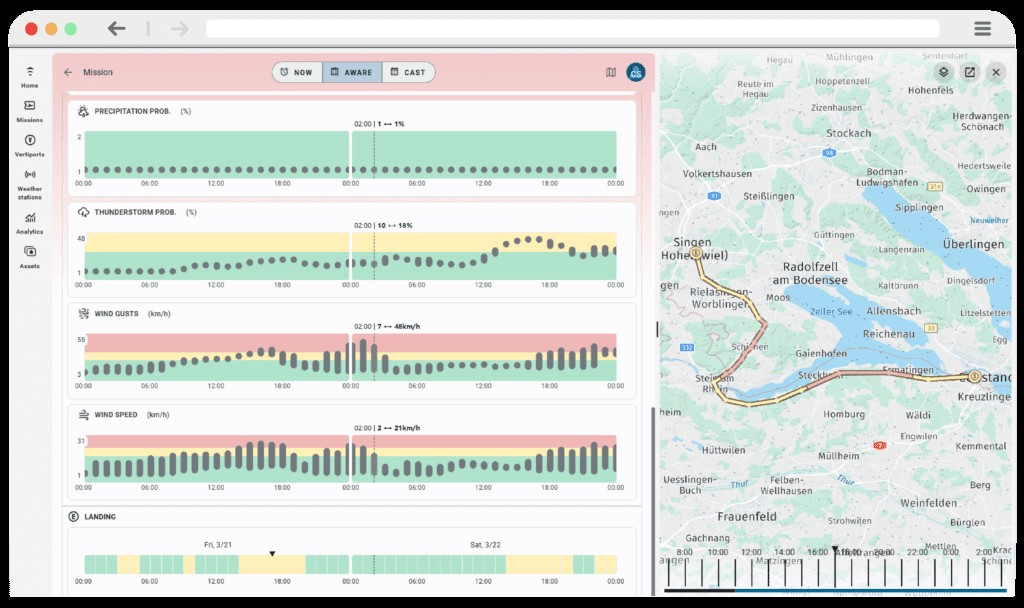
\includegraphics[width=0.9\textwidth]{images/NOVA.jpg}
%  \caption{NOVA Platform interface for mission planning and weather tools.}
%  \label{fig:nova}
%


\section{Project Methodology and Work Plan}

\subsection{Development Approach}

The internship followed a structured yet flexible approach inspired by Agile principles. Rather than relying on a rigid predefined plan, the work progressed incrementally through data analysis, KPI definition, implementation, testing, and validation. Each stage was reviewed and refined based on practical findings and technical feedback.

The first steps focused on understanding the OEE methodology, system architecture, and available data. The work then progressed toward data preparation, KPI computation, validation, and reporting. Regular exchanges with the company supervisor and updates to the academic supervisor ensured continuous alignment with the project objectives.
\subsection{Project Timeline}
The internship spanned a total of six months, from March 2026 to August 2026. The project was divided into clear, consecutive phases to ensure efficient progress and a logical development workflow. The following timeline outlines the major milestones and activities:

\begin{figure}[H]
  \centering
  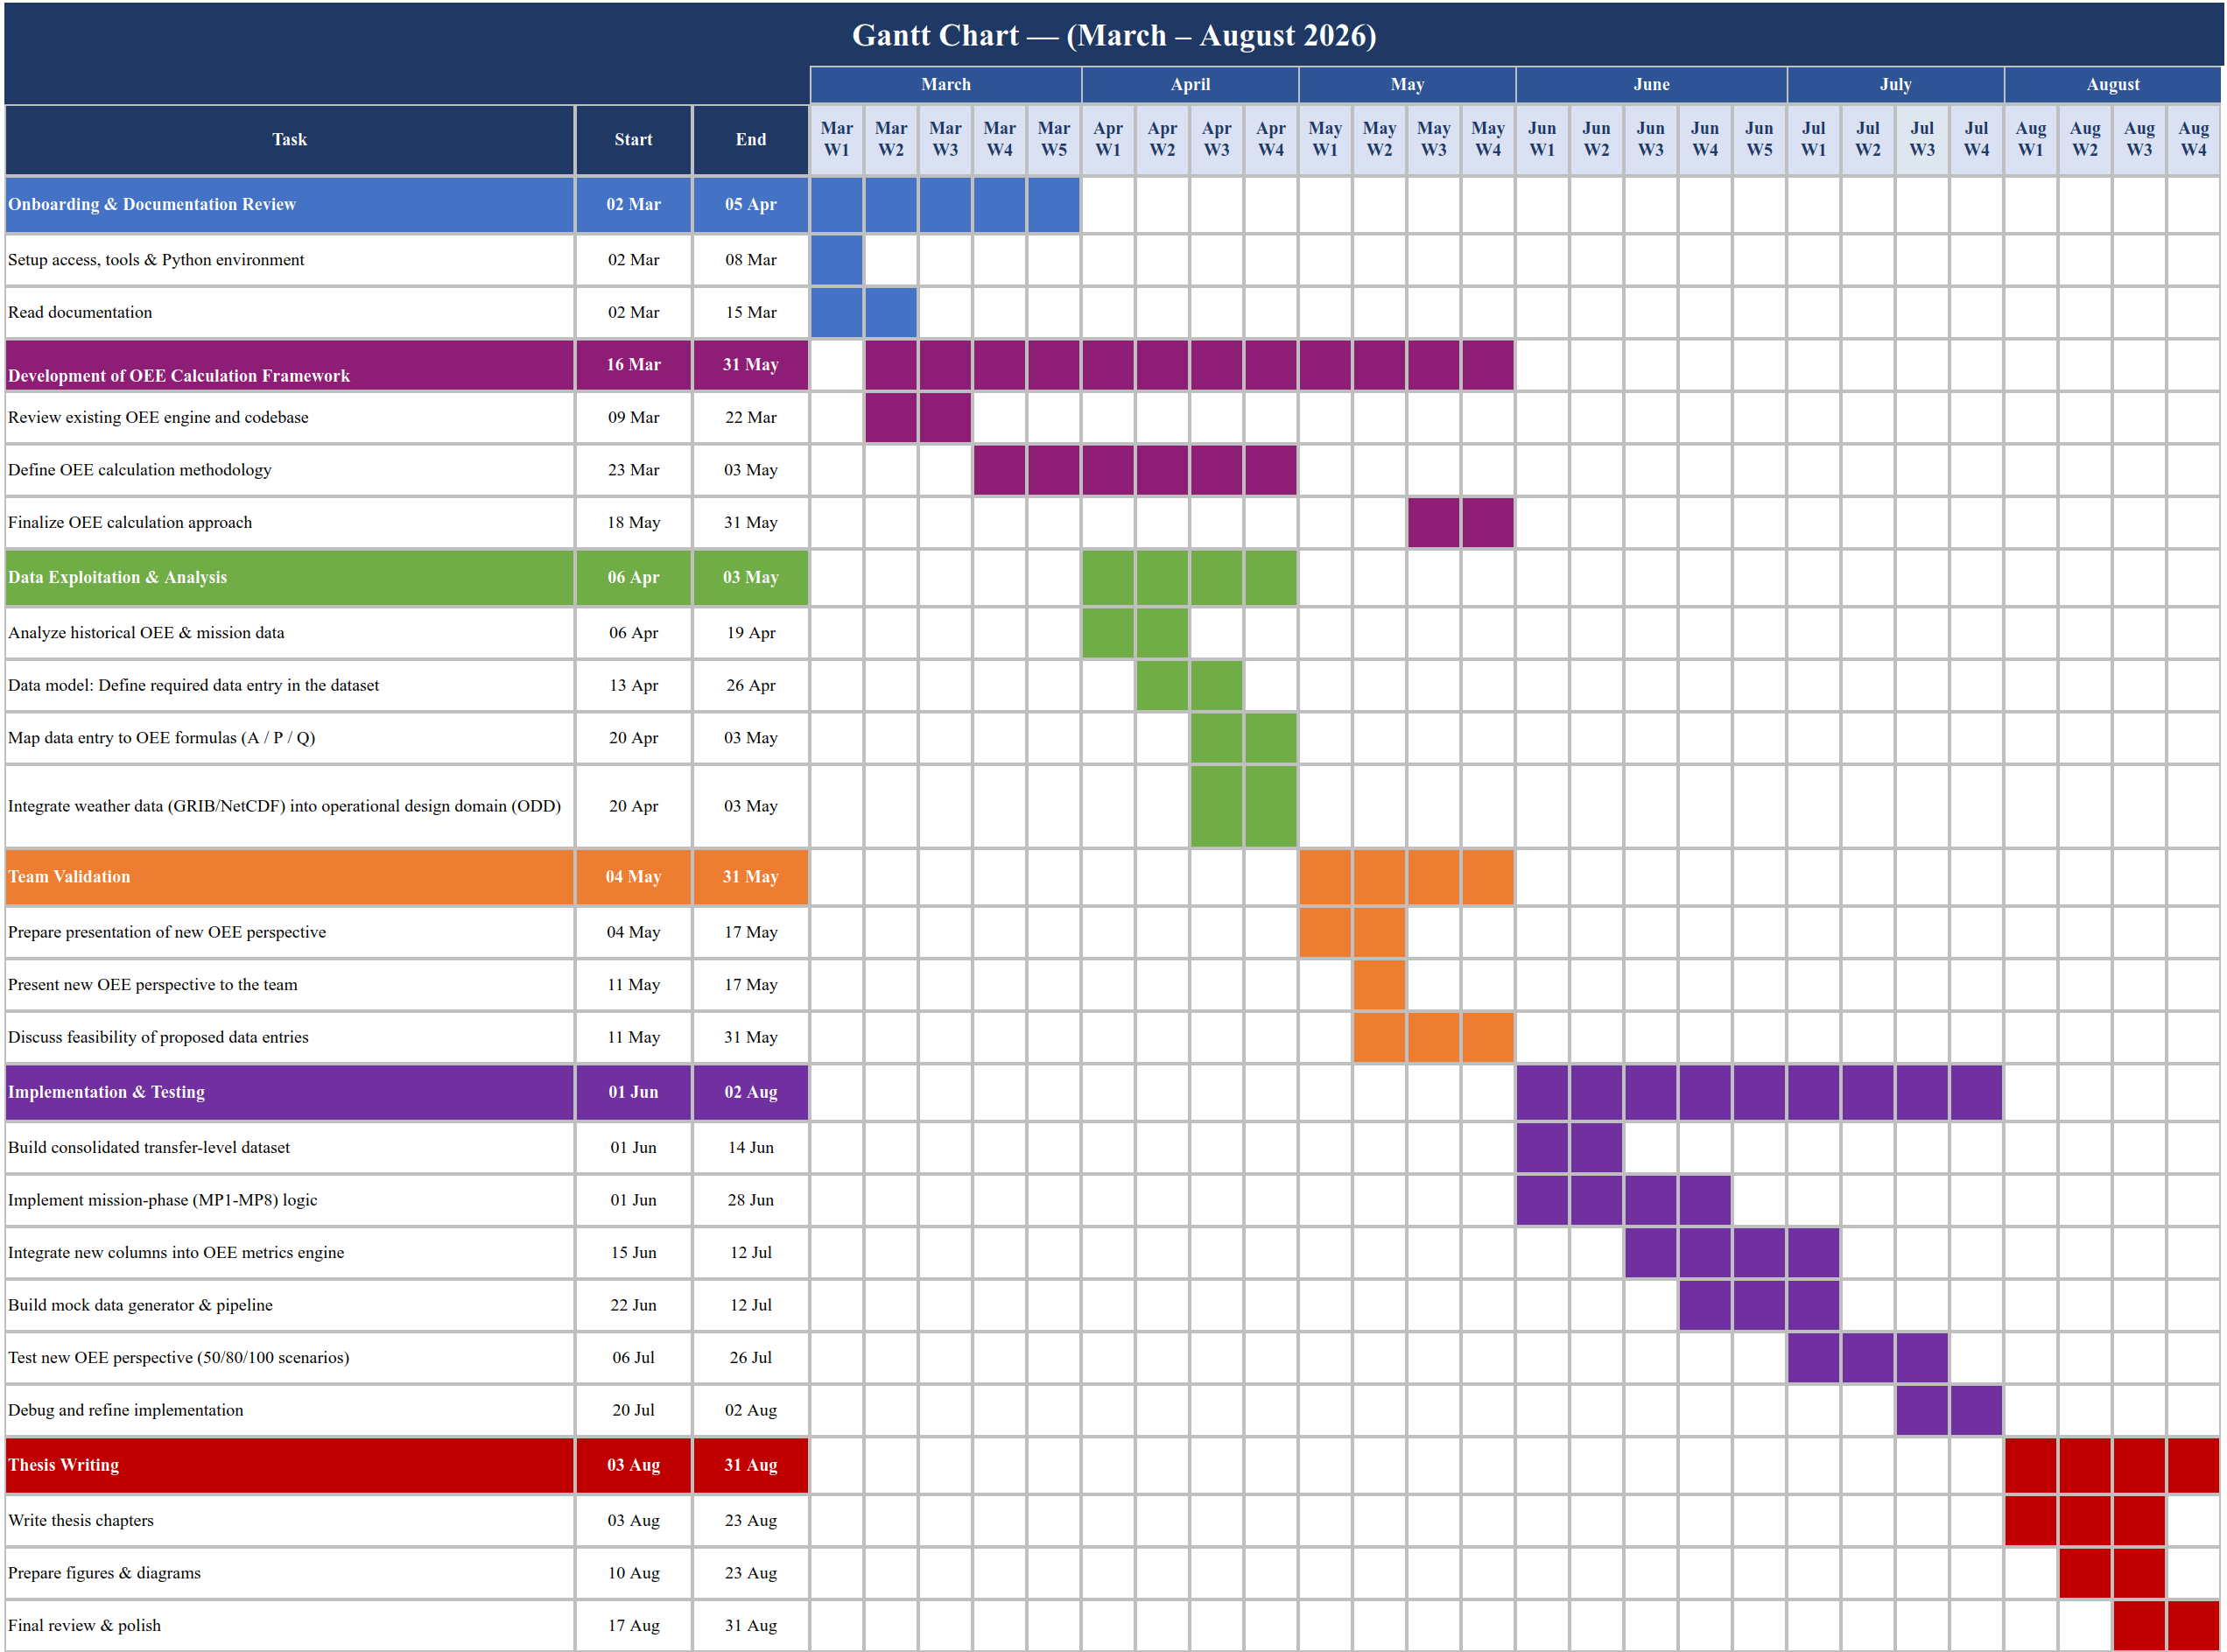
\includegraphics[angle=90, width=1\textwidth]{images/GanttChart.png}
  \caption{Gantt Diagram}
  \label{fig:gantt}
\end{figure}

\section{Conclusion}

This chapter established the industrial and theoretical foundations of the work. It presented TII KAMAG, the autonomous yard-logistics system, its operating environment, system actors, transfer workflow, mission hierarchy, architecture, and data sources. It also showed that operational effectiveness depends on technical performance, mission variability, human supervision, traffic, and environmental conditions.

The review of \gls{oee} showed that Availability, Performance, and Quality provide a useful structure for measuring industrial effectiveness. However, classical \gls{oee} was developed for stable manufacturing systems with fixed cycle times. Autonomous yard vehicles operate under variable conditions and generate specific events, such as interventions, disengagements, autonomy limitations, and ODD-related exclusions. Existing autonomous-vehicle \gls{kpi}s, reliability metrics, and capability indices provide valuable information, but they do not combine these aspects into one integrated measure.

These findings define the research gap addressed by this work. \textbf{An adapted \gls{oee} framework is required for autonomous yard logistics}. The framework must account for variable mission durations, autonomy-specific losses, supervision requirements, and ODD-related constraints. The following chapter presents its measurement unit, time hierarchy, adapted \gls{oee} factors, loss classification, \gls{odd} treatment, and complementary indicators.